\chapter{Signal conditioning stage design} \label{app:if}

In this appendix, the design of the additional signal conditioning stage is described. This stage serves the purpose of conditioning the signals from the radar control board to the microcontroller (MCU) analogue-to-digital (ADC) converter.

\section{Circuit design}

The main purpose of the circuit, as explained in \cref{sec:signal-conditioning-additional-if-stage-design}, is to drive the ADC input with a properly scaled and amplified intermediate frequency (IF) signal and with a low-low impedance source. For that matter, a design based on an operational amplifier (OA) is carried out. The circuit must be able to provide a $3.3/2 = \SI{1.65}{\volt}$ DC-shift.

Parting from recommended ADC buffer design guidelines from Texas Instruments \cite[p.~17]{TexasInstruments2022} and \cite{Franco2014}, a common circuit used for this purpose is laid out in the multi-purpose simulation software Keysight ADS. The circuit is shown in \cref{fig:if_cir}.

\begin{figure}[h]
	\centering
	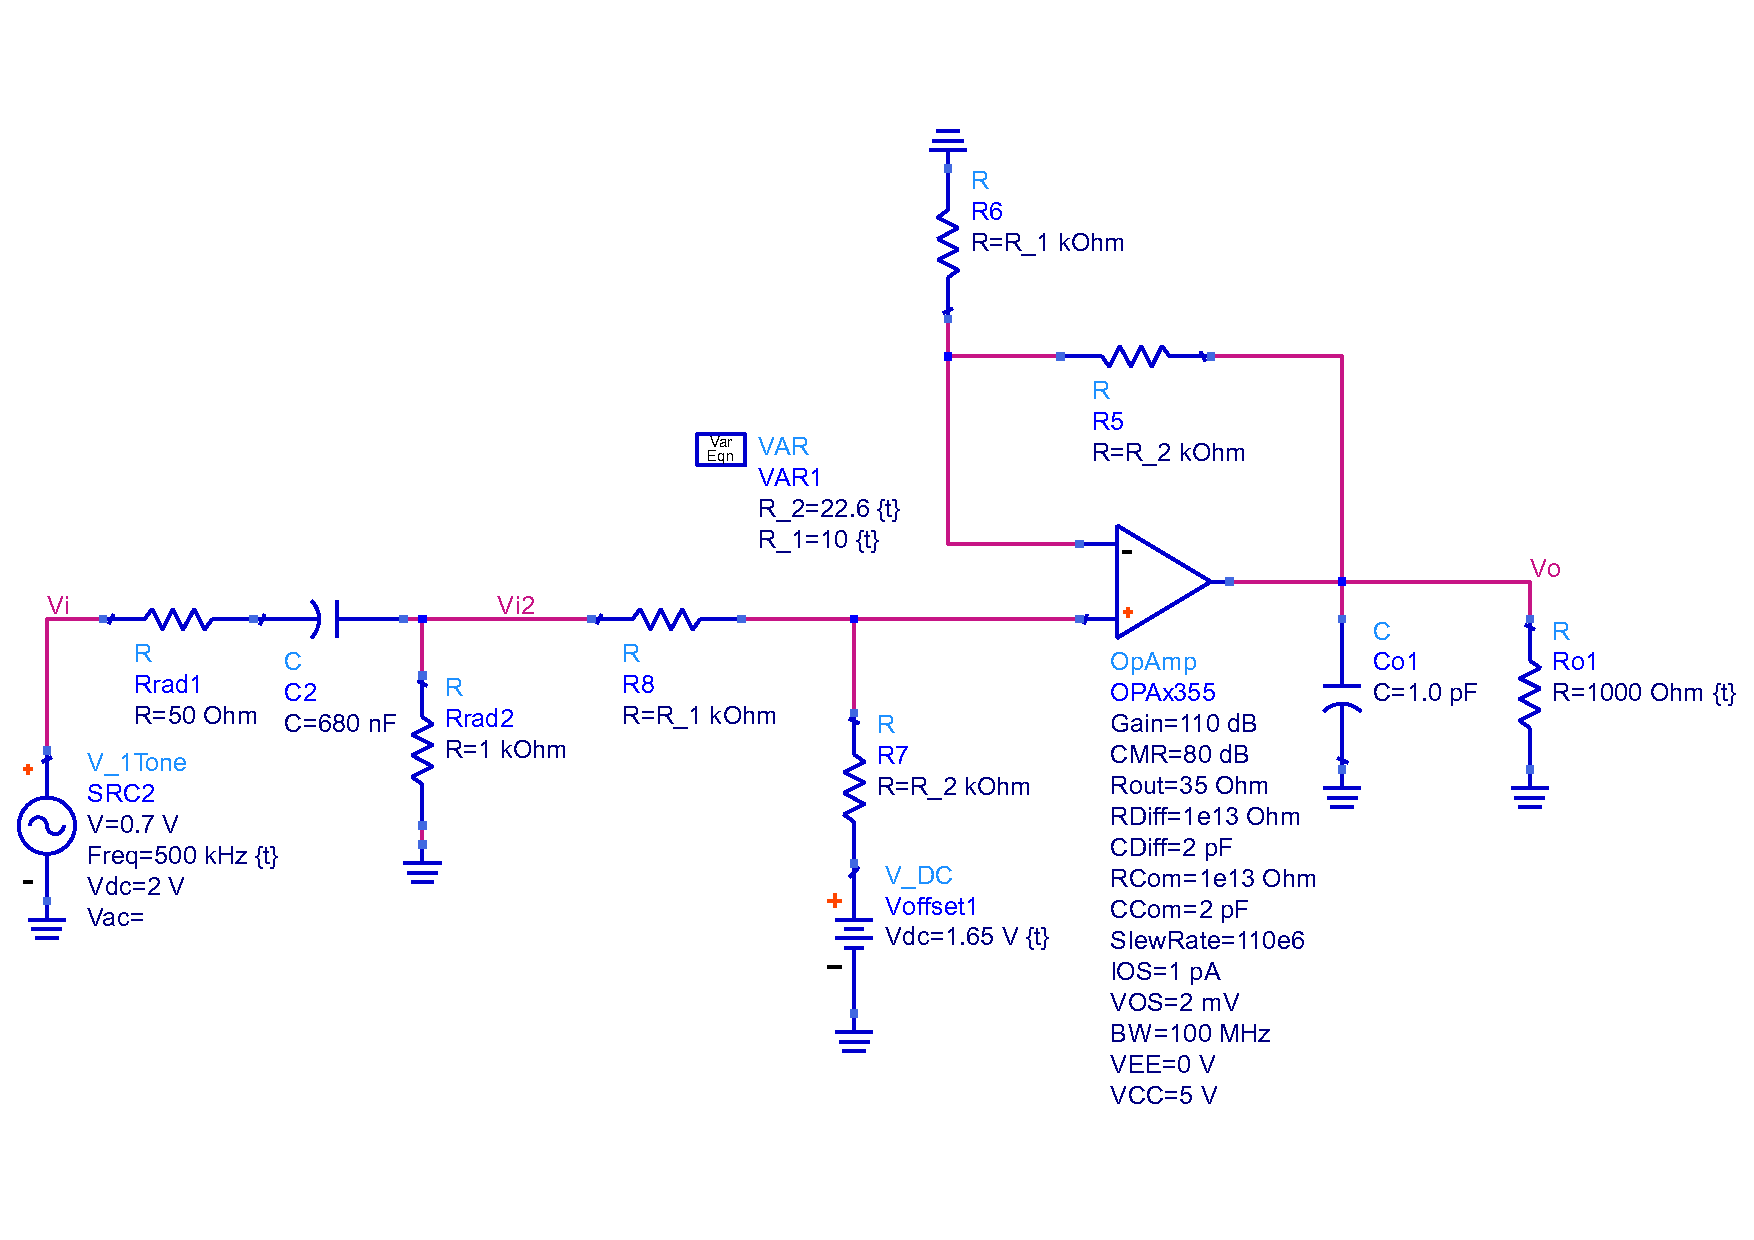
\includegraphics[width=\linewidth]{if/ads_circuit.pdf}
	\caption{Circuit of the IF stage signal conditioning step containing an OA. \textit{V\_DC} is the DC-shift provided. The resistors of the feedback networks are responsible of setting the gain configuration. Two configurations of this circuit are used, one for every component of the IF signal from the baseband radar.}
	\label{fig:if_cir}
\end{figure}

The OA used in the driver can be any op-amp having a GBW that is able to accommodate all the incoming signal from the filter:
\begin{equation}
	GBW_{OA} \ge \frac{BW_{f}}{G}
\end{equation}
being $G$ the gain of the OA and $BW_{f}$ the bandwidth of the filter.


\subsection{Gain configuration}
The values of $R_1, R_2, R_3, R_4$ are used to set the gain $G$ of the OA.
In this particular application a pure AC waveform of \SI{1.4}{Vpp} needs to map to a waveform of \SI{3.3}{Vpp}, thus:
\begin{equation}
	G = \frac{3.3}{1.4} = 2.357 %TODO: change to correct values
\end{equation}
and after analysing the circuit feedback loops:
\begin{gather}
	G = \frac{R_4}{R_1} \frac{R_1+R_2}{R_3+R_4}\\
	R_1 = R_3, R_2=R_4\\
	G= \frac{R_4}{R_1} %TODO: change to correct values and calculations
\end{gather}
after giving a fixed value of \SI{10}{\kilo\ohm} to $R_1$:
\begin{equation}
	G \cdot \SI{10}{\kilo\ohm} = R_4 = \SI{23.57}{\kilo\ohm} %TODO: change to correct values and calculations
\end{equation}
By allowing for some margin at the extrema of the output, and considering that there aren't commercial resistors of the computed value, the closest value of \SI{22.6}{\kilo\ohm} has been chosen for $R_4$. This value corresponds to the closest E12 value available, which is the preferred series of values for electronic components \cite{IEC2015}. Leaving some margin also lessens the impact of the noise floor of the ADC.
At the output of the OA, a small capacitor is placed in parallel to allow for smooth voltage output and high-frequency voltage spikes suppression.

The chosen OA has been OPA2354AIDDA \cite{TexasInstruments2014}, because it has a sufficiently large bandwidth for the application (suitable GBW) and there is readily available stock at the laboratory. This is chosen so that the design is capable of working for input signals frequencies of well over the required 1 MHz bandwidth. Additional capabilities such as a stage to convert from differential format IF signals to single-ended has also been added in case working with other radars require it.

\section{Schematic}

The design is materialised with the corresponding components and connectors in a schematic sheet. The design features several components such voltage regulators to drive the OAs and SMA connectors to input and output signals. The schematic for this circuit is shown in \cref{fig:sch_if}.

\begin{figure}[h]
	\centering
	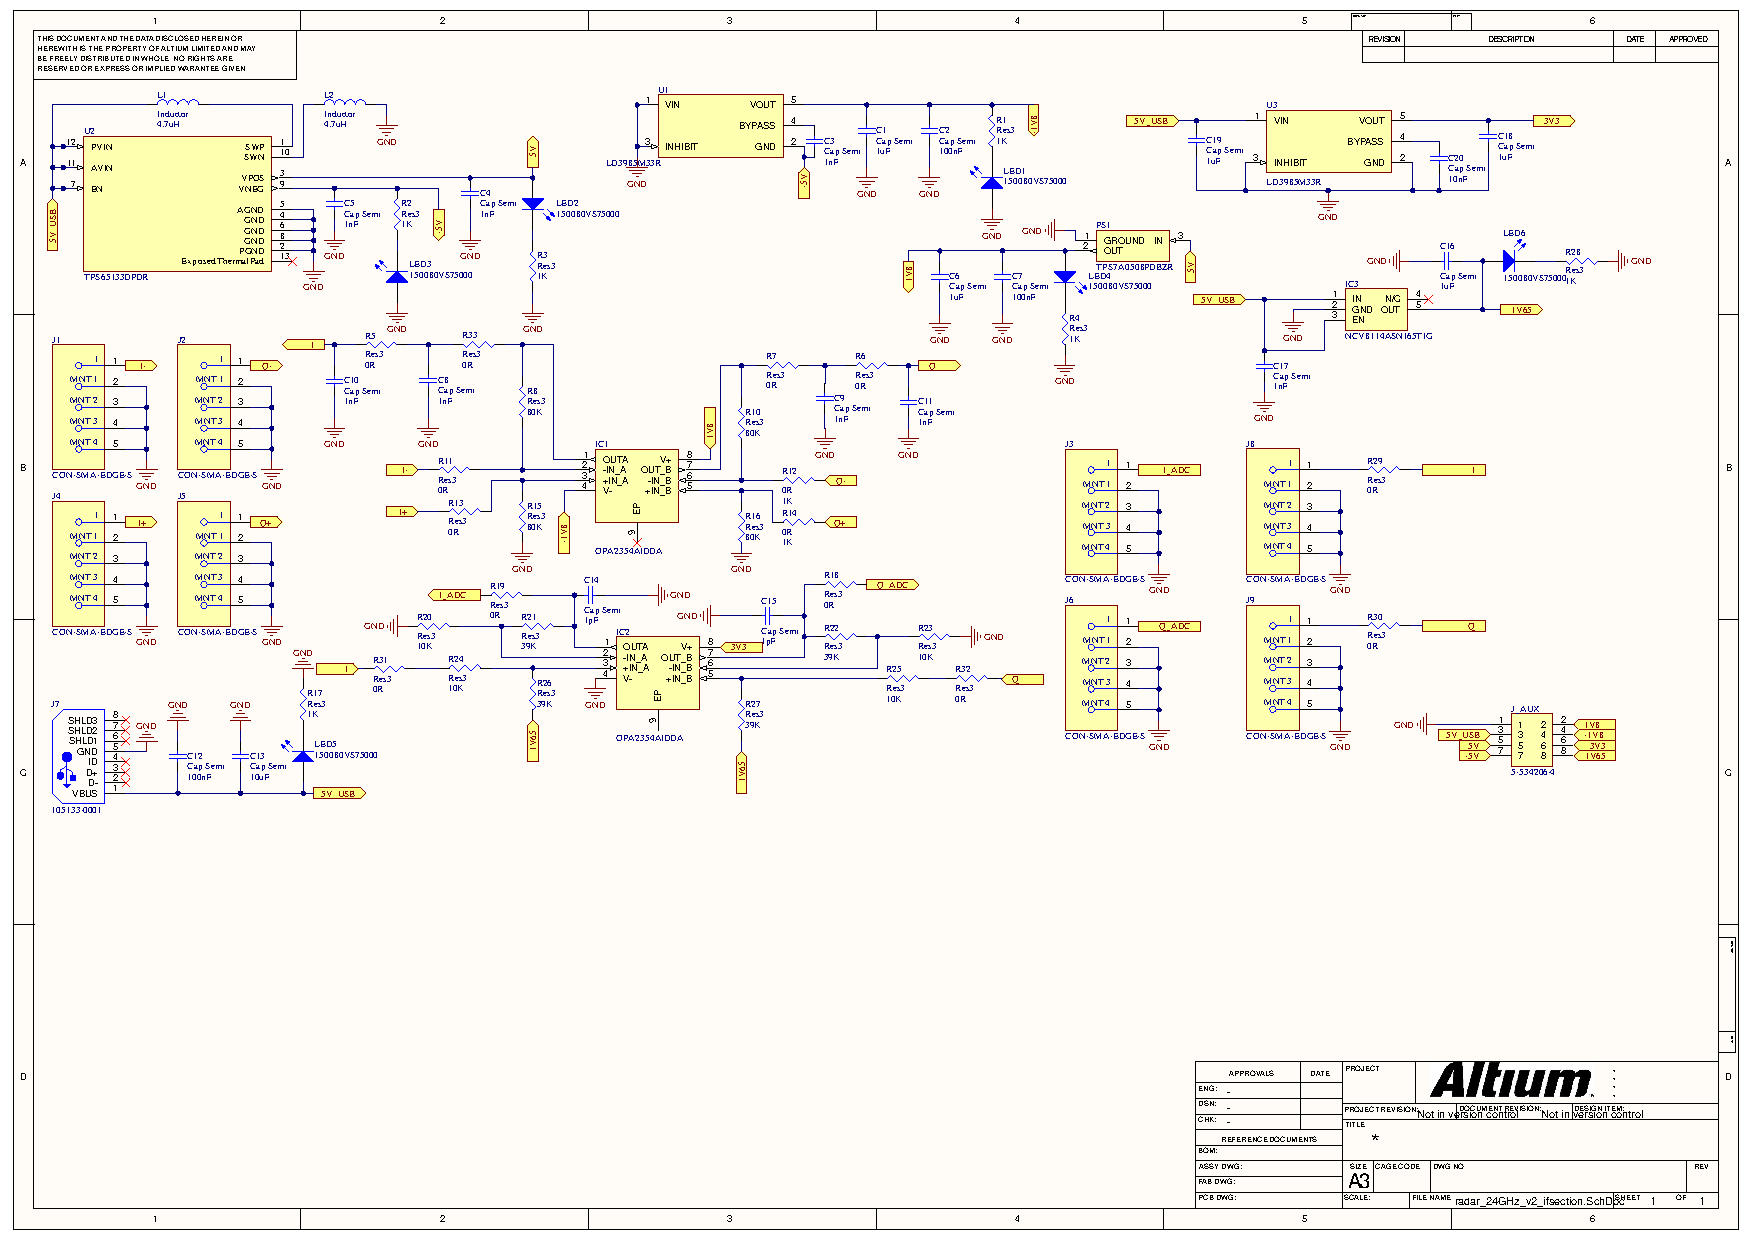
\includegraphics[width=18cm, angle=90]{sch/if.pdf}
	\caption{Schematic of the IF stage PCB. Two pairs of OAs (4 total OAs) are responsible for the gain and shifting characteristics of the stage. Some resistors might show a value different to the circuit: when assembling the PCB, the correct value for the resistors was installed. This is due to allow different board configurations for testing due to the component footprints remaining the same.}
	\label{fig:sch_if}
\end{figure}

\section{Layout}

The schematic components and nets are laid out in a PCB layout. The corresponding connecting nets and components are routed and the PCB layout is designed. The layout for this PCB is shown in \cref{fig:lay_if}. A 3D render of the board can be seen in \cref{fig:lay_if_3d}

\begin{figure}[h]
	\centering
	\includegraphics[width=\textwidth]{lay/pcb_if.pdf}
	\caption{Layout of the IF stage PCB. The red traces represents routing in the Top Layer. The blue traces represents routing in the Bottom Layer. Vias are represented as grey holes.}
	\label{fig:lay_if}
\end{figure}

\begin{figure}[h]
	\centering
	\includegraphics[width=0.7\textwidth]{3d/pcb_if}
	\caption{3D render of the IF stage PCB from the top.}
	\label{fig:lay_if_3d}
\end{figure}


